\documentclass{article}
\usepackage{amsmath}
\usepackage{graphicx} 
\usepackage{framed}
\usepackage[utf8]{inputenc}
\usepackage[a4paper, total={5.5in, 8.0in}]{geometry}
\usepackage[english]{babel}
\usepackage[document]{ragged2e}

\title{Digital Derby Report}
\author{Eric Pu and Leon Kalish \\ Ms. Wong}
\date{November 2019}

\begin{document}

\maketitle

\graphicspath{ {./images/} }

\newpage
\tableofcontents
\newpage

\begin{figure}[h]
\centering
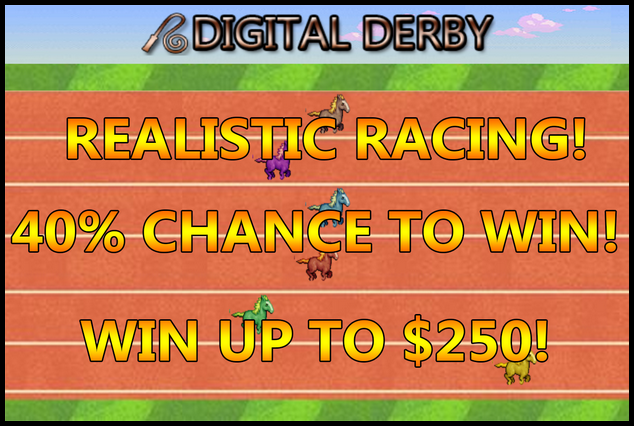
\includegraphics[width=6.5cm]{images/poster.png}
\caption{Poster}
\end{figure}

%TODO explain the pitch and how it created
\section{Game Information}
{
On your marks… get set… go! Horse racing is an exhilarating and fun way to either win it big or lose it all. Unfortunately, horse racing is quite a difficult game to get into as a new player. Newbies are overloaded with stats, records, and all kinds of external factors. Some people wish that horse racing could be as simple as betting on your favorite color. Fortunately, this new casino game lets you do just that! Digital Derby brings the fun of horse racing to the casino, making the game simple enough for anyone to get started! With a 40\% chance to win and a jackpot of \$250, Digital Derby is the best way to win big while having a whole lot of fun.
\vspace{5mm}

\section{Rules}
{
\begin{enumerate}
    \item Player chooses three horses on the betting screen: the horses they believe will come in first, second, and third.
    \item Each horse is functionally identical, meaning they all have an equal chance to win.
    \item The payout is awarded based on which of the guesses were right. Guessing higher places correct will reward more than lower places (i.e. getting first place right has higher payout than third place). 
\end{enumerate}

}



}


\vspace{2ex}
\section{Game Mechanics}
{
While Digital Derby may seem like a fundamentally simple game from the player's perspective, that is because many of the game's internal mechanics are obfuscated to minimize the barrier of entry. Underneath its colorful exterior, Digital Derby functions off of many complex mechanics which ensure a realistic and fair racing experience.
\vspace{2ex}

In Digital Derby, all six of the horses are functionally identical, and are all implemented the same way. The game works by generating a new velocity after every time interval. The time interval is random, and is between 150 and 300 frames. There are 60 frames per second.

\vspace{2ex}

Each race begins with every horse generating a new velocity. To simulate the effect of acceleration, the horses transition into their new velocity for 30 frames. The horse’s velocity changes by the difference in velocities / 30, so that the horse’s velocity will be equal to the newly generated velocity after half a second. The velocity is randomly chosen between a range of 2.5 and 4.5 pixels per frame.

\vspace{2ex}

When the horses reach a certain position away from the left side of the screen, the camera begins to pan to the right. This is used to show a scrolling effect similar to real horse race coverage.

\vspace{2ex}

The race ends when all the horses pass the finish line. The finish line begins at 5000 pixels right of the screen. The finish line and camera move at the velocity of the fastest horse, to simulate how cameras follow the fastest horse in real races. Once the finish line is within 1050 pixels from the left side of the screen, it can be seen by the player. 

\vspace{2ex}
}

\begin{figure}[h]
\centering
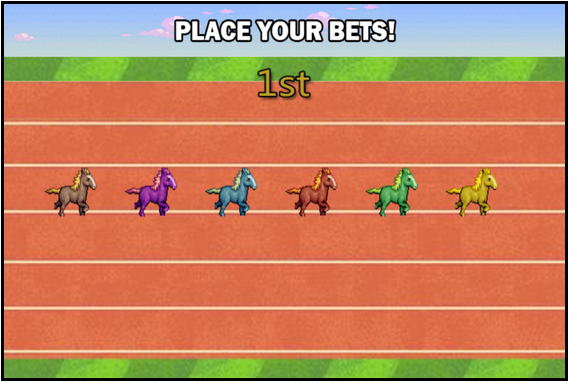
\includegraphics[width=6.5cm]{images/placebets.png}
\caption{Betting Screen}
\end{figure}

\begin{figure}[h]
\centering
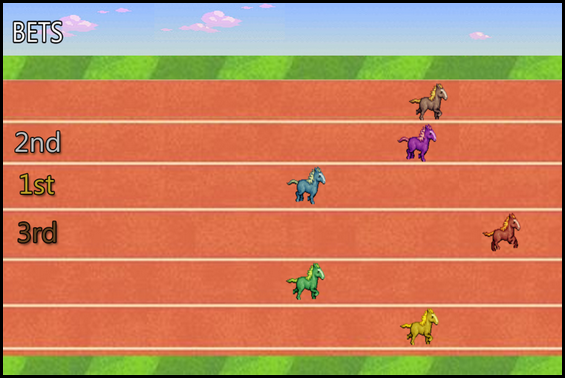
\includegraphics[width=6.5cm]{images/racescreen.png}
\caption{Racing Screen}
\end{figure}


\section{Calculations}
{
All 6 horses being raced have the same odds of finishing in first, second, or third, so for all further calculations it is implied that there is no bias or tendency towards a certain horse.

\vspace{2ex}

The general formulas used are uniform probability formulas, as the only probability changing factors are the number of horses available. 

\vspace{2ex}

To solve for the rest of our outcomes, we must first calculate the probability of scoring all three guesses correctly. 

\vspace{2ex}
\subsection{All Three Correct}
{
The first guess has a 1/6 chance of being correct. The second guess will have a 1/5, as there are five horses remaining at that point. The third guess will have a 1/4 chance. To find the odds of getting all three correctly, we simply multiply them together.

\begin{equation}
    \begin{split}
        P(1,2,3) &= (1/6)(1/5)(1/4)\\
        &= 1/120\\
        &\simeq 0.8\overline{3}\%
    \end{split}
\end{equation}
}

Using this calculation, we find the probability of all three correct, which we will then use for finding the probability of outcomes with two correct guesses. There are three of these outcomes: Place 1 and 2 correct, 1 and 3 correct, and 2 and 3 correct. All of these outcomes have an equal chance of occurring.

\vspace{2ex}
\subsection{Two Correct}
{
To calculate these outcomes, we use the same process as before with the first and second guess, but we must also subtract the chance of getting all three correct to prevent double counting.

\begin{equation}
    \begin{split}
        P(1,2) &= (1/6)(1/5) - P(1,2,3)\\
        &= 1/40\\
        &= 2.5\% \\
    \end{split}
\end{equation}
}

\vspace{2ex}
P(1,2), P(1,3), and P(2,3) all have an equal chance of occurring, so we will only need to make one calculation.

\vspace{2ex}
\subsection{One Correct}
{

Now, we can find the probability of getting only one guess correctly. There are three of these outcomes: 1, 2, and 3. 

\vspace{2ex}

There’s a 1/6 chance of getting a single guess correctly, but we must also subtract the chances of getting two or three correct to prevent double counting. We subtract the chance of getting two correct twice, as there are two outcomes which involve getting the first guess and another guess right. We also subtract the chance of getting all three correct.

\begin{equation}
    \begin{split}
        P(1) &= (1/6) - 2P(1,2) - P(1,2,3)\\
        &\simeq 10.8\overline{3}\%
    \end{split}
\end{equation}
}

\subsection{None Correct}
{
With these calculations, we are now able to calculate the probability of getting none of the guesses right. This can be found using indirect method.

\begin{equation}
    \begin{split}
        P(None) &= 1 - 3P(1) - 2P(1,2) - P(1,2,3)\\
        &\simeq 51.\overline{6}\%
    \end{split}
\end{equation}
}
\vspace{2ex}
We now have the probability of each of the 8 possible outcomes.

\begin{equation}
    \begin{split}
        P(1) &\simeq 10.8\overline{3}\% \\
        P(2) &\simeq 10.8\overline{3}\% \\
        P(3) &\simeq 10.8\overline{3}\% \\
        P(1,2) &= 2.5\% \\
        P(1,3) &= 2.5\% \\
        P(2,3) &= 2.5\% \\
        P(1,2,3) &\simeq 0.8\overline{3}\% \\
        P(None) &\simeq 51.\overline{6}\% \\
    \end{split}
\end{equation}
}

\vspace{2ex}

If you recall, we stated in the poster that players have a 40\% chance to win in Digital Derby. The chance of winning any payout can be found by subtracting P(None) from 1, resulting in a 48.4\% of winning: a number that is actually higher than what is advertised.

\vspace{26ex}

\section{Theoretical Expected Value}

\begin{figure}[h]
\centering
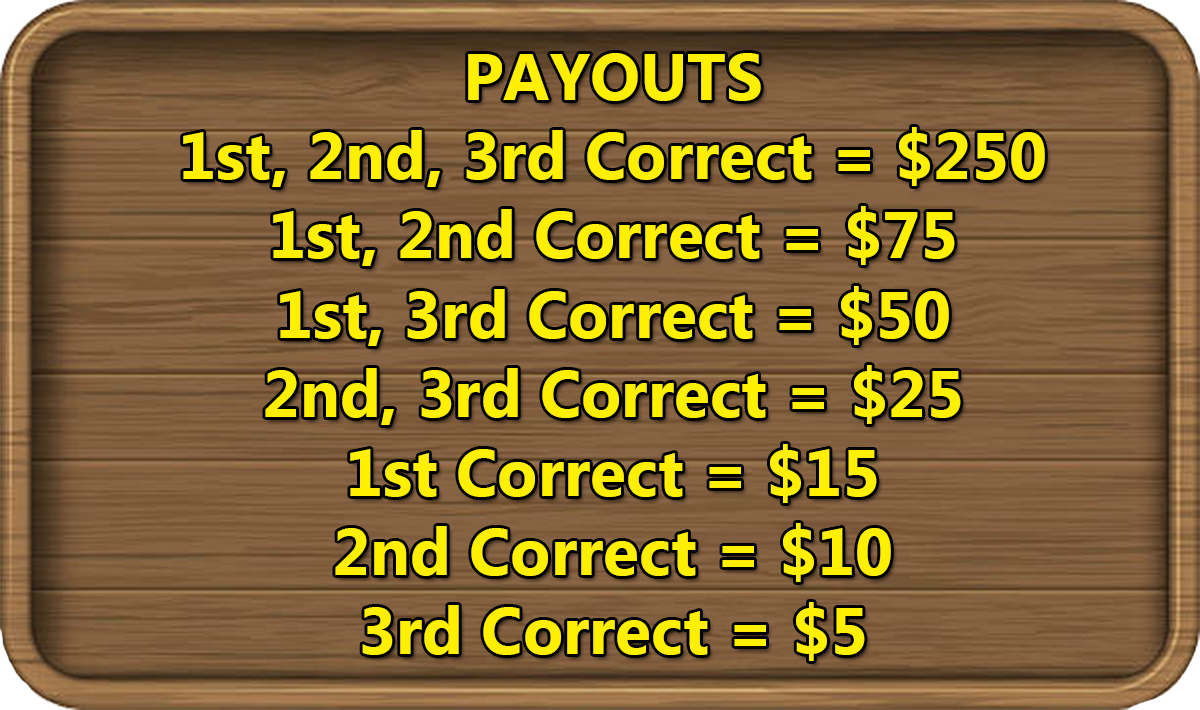
\includegraphics[width=6.5cm]{images/payouts.png}
\caption{Payouts}
\end{figure}

{With the probability of each outcome, the expected value can now be calculated. To do so, we simply multiply each payout by the probability of it occurring.
\vspace{2ex}

\begin{equation}
    \begin{split}
        E(X) &= (0)(.517) + (250)(.0083) + (25)(.025) + (50)(.025)\\ &+ (75)(.025) + (5)(.1083) + (10)(.1083) + (15)(.1083)\\
        &\simeq 9.08 
    \end{split}
\end{equation}
\vspace{2ex}

This value indicates that one round of Digital Derby has an expected payout of \$9.08. Using this value, we can also find the average profit/loss.

\begin{equation}
    \begin{split}
        P/L &= E(X) - Cost\\
       &= \$9.08 - \$10.00\\
       &= -\$0.92
    \end{split}
\end{equation}
\vspace{2ex}

Therefore, a player can expect to lose 92 cents each time they play Digital Derby. This represents a profit margin of 9.2\% for the operators of the game. This is enough for the game to be both profitable for its operators and fair for its players.
}

\section{Data Analysis}
{
Throughout the two casino days, we were able to collect 100 pieces of data. Unfortunately, this was an insufficient sample size to do any proper data analysis. 400 additional pieces of data were generated by running the game, resulting in a total of 500 trials.

\vspace{2ex}

The first question we had with Digital Derby was if each horse’s odds of winning were equally likely. To do so, we simply counted how many times each horse finished in the top 3. These were the results. 


\begin{figure}[h]
\centering
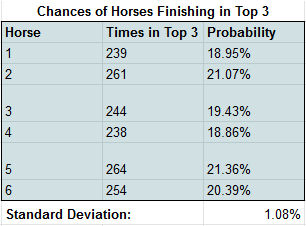
\includegraphics[width=6.5cm]{images/chancetop3.png}
\caption{Table with top 3 finishes}
\end{figure}

\vspace{2ex}

The first question we had with Digital Derby was if each horse’s odds of winning were equally likely. To do so, we simply counted how many times each horse finished in the top 3. These were the results. 

\begin{figure}[h]
\centering
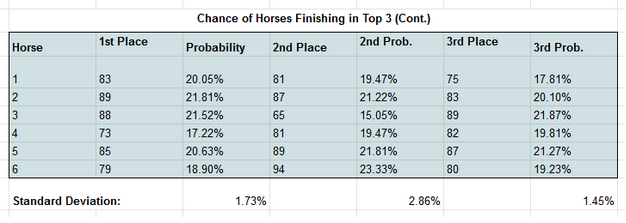
\includegraphics[width=10cm]{images/chancetop3expanded.png}
\caption{Expanded Top 3 Finish Table}
\end{figure}

As you can see, the probabilities are fairly similar once again. This proves that each horse has an equal chance at scoring first, second, or third place. This data is integral for verifying that Digital Derby is completely fair, and enables our second stage of data analysis.

\vspace{2ex}

Now, we can analyze the probabilities of each possible payout.

\vspace{5mm}
\begin{figure}[h]
\centering
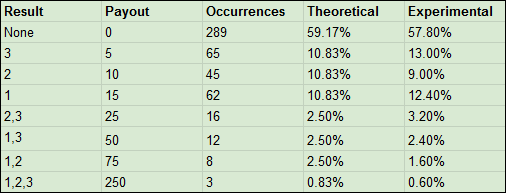
\includegraphics[width=8.5cm]{images/oggameresults.png}
\caption{Game Result and Payout Percentage}
\end{figure}

For the most part, our theoretical probabilities are close to the experimental probabilities. While it may seem that there is a large difference for certain results, such as 1, 1 and 2, or 2 and 3, the problems can be resolved by looking at the sum of similar outcomes with the same probability. For instance, if we add up the probabilities of all outcomes with one correct guess, we get 34.40\% for the experimental, and 32.49\% for the theoretical. For two correct guesses, we get 7.2\% for the experimental and 7.5\% for the theoretical. These combined probabilities are much closer than the individual probabilities. 

\vspace{2ex}

With the calculations for each individual payout complete, we can do an analysis on the game overall. 

\begin{figure}[h]
\centering
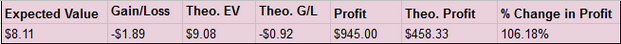
\includegraphics[width=10cm]{images/ogprofit.png}
\caption{Profit/Loss Table}
\end{figure}
There is quite a large difference between our experimental and theoretical results. Using the numbers from the previous table, the average payout of Digital Derby in the sample is \$8.11 — 97 cents less than the theoretical amount calculated before. 

\vspace{2ex}

The profit was calculated by simply taking the average payout and multiplying by the number of trials (500). Theoretical profit was found in the same way, but using the theoretical payout instead. 

\vspace{2ex}

Percent change in profit was found by finding the difference in the experimental and theoretical profits, divided by the theoretical profit. The value of 106.18\% means that our experimental profit is more than double that of the theoretical: a massive difference.

\vspace{2ex}

The likely cause of this disparity is the small sample size of 500. As we saw earlier, the probabilities of each outcome were mostly similar to that of what we expected. However, a small difference in these probabilities can result in a large difference in profit. For example, while the probability of the jackpot being slightly lower than the theoretical might not seem like a big deal, having one less jackpot has a huge impact on the average payout -- even across 500 trials.
}
\section{Simulation - 10\textsuperscript{6} trials}
{
Unfortunately, given the high margin of error that comes with a sample size of 500, we are forced to find other avenues of obtaining data. One easy way to mitigate this problem is to use a program that can simulate the mechanics of Digital Derby, allowing us to easily generate millions of points of data. Using a simulation will get us much closer to our calculated values. 

\vspace{2ex}

For the simulation, we used a simple program written in Python. The code for the simulation can be found here: https://repl.it/repls/FloralwhiteRowdyTechnicians. 

\vspace{2ex}

For our second data sample, we decided to use a trial of 1,000,000 data points. Here are the results: 
\vspace{6ex}
\begin{figure}[h]
\centering
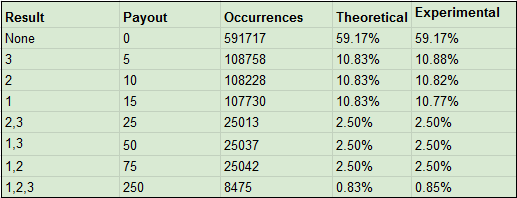
\includegraphics[width=8.5cm]{images/gameresults1m.png}
\caption{Results for 1,000,000 Simulations}
\end{figure}

For the individual payouts, we can see that the experimental probabilities are much closer to the theoretical probabilities. In fact, the probabilities for all outcomes involving 2 correct guesses are equal, as well as the probability of getting none correct. Furthermore, the difference between the sum of theoretical and the sum of experimental probabilities for getting one guess correct is only .02\% (32.49\% vs 32.47\%)

\vspace{2ex}

\begin{figure}[h]
\centering
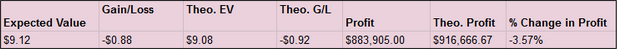
\includegraphics[width=10cm]{images/profittable1m.png}
\caption{Profit/Loss Table at 1,000,000 Simulations}
\end{figure}
\vspace{2ex}
When it comes to the overall table, we see much better results as well. While the first data set showed a 106.18\% increase in profit from what we expected, this sample of one million cases shows a -3.57\% change instead. This number is much closer to our ideal change of 0\%. In terms of the expected values, we see the two values are also very similar, with a difference of only 4 cents (as opposed to the difference of 97 cents found in the first sample).

\vspace{2ex}

With this simulation, our hypothesis that our initial data was skewed by a low sample size was proven correct. With 2000 times the sample size, our data is now much closer to what we expected from our calculations.
}

\section{Reflections}
{
\subsection{Bias}
{
Perhaps the greatest advantage of programming Digital Derby is the certainty that comes with each play. Since there are no external factors that can influence the results of the game, as each horse is truly random, there is no potential for bias. This ensures that all results are consistent, and vastly increases the reliability of our data.
}
\subsection{Eric}
{
Personally, I believe that there were both pros and cons with Digital Derby. The main issues with the game stem from the presentation. I believe that our panel was simply not alluring or flashy enough, hence why we were only able to get 100 pieces of data during our two casino days. The main drawback came from my small laptop screen, which made it difficult to stand out from the other games. 

\vspace{2ex}

One way we could’ve mitigated this problem would be using a larger display, such as a desktop monitor. This would’ve not only made it easier for spectators to observe their bets, but also would’ve brought more players to our game.

\vspace{2ex}

Obviously, our game stood out from the others in one major way: the game was digital, rather than physical. Of course, having to program a game from scratch took a lot of time; likely more than producing a physical one instead. However, we thought that differentiating ourselves from the rest and creating a unique digital experience would result in a far more interesting product than simply doing a physical board or card-based game instead. Regardless, I believe making the game digital paid off, as many players enjoyed rooting for their favorite horses. 

\vspace{2ex}

The primary issue with the game was the amount of time it took to complete each round. It took approximately 30 seconds to complete one round originally, which was far more than the few seconds that our peers’ games took. We eventually reduced that time to approximately 22 seconds instead, which did speed up the betting process a bit, while still keeping the game intense with the chance of comebacks. Another issue was the lack of player interaction. The only thing players are tasked with doing is selecting their three horses. While this reduces the barrier to entry, it also reduces their ability to interact with the game and thus makes the entire experience less enjoyable. 

\vspace{2ex}

As for the other games, I felt that most of them were very impressive. One notable example was Super Buzz, which had an incredibly intricate and colorful board. Perhaps the most important component of a casino game is the presentation, and having such a flashy board to captivate players ensures that they will play again. The mechanics of the game were also interesting, allowing players to choose their own risk levels, while also offering many options when it comes to placing your bets.

\vspace{2ex}

Another notable game was Disarm the Bomb. The game was definitely flashy, with its oversized dice and well-arranged board. I particularly enjoyed the way this group allowed players to choose their own risk, by giving them the option of double or nothing. This simple mechanic adds a lot of depth to a game, and makes winning a whole lot more interesting. 

\vspace{2ex}

Overall, this casino assignment was quite enjoyable. I learned quite a few things about the importance of presentation, and how to properly attract people to your product. I also learned about how to collect and analyze data, and the power of having a large sample size. 

\vspace{2ex}

If I could change anything about Digital Derby, I would make the game a lot more visually appealing. Simply having a larger display to show potential players the game would’ve been a huge advantage. Also, giving players the ability to choose their own risks would’ve vastly increased the depth of the game. Digital Derby focused primarily on the experience of the game, rather than the payout. Adding more of an emphasis to the payouts, through more advanced game mechanics, would’ve made the game a lot more fun. 

}
\subsection{Leon}
{
%plunder, digital derby, liscence to win, lucky ducky, super buzz, disarm the bomb
Digital Derby does an excellent job of simulating what a casino would be like, with the colorful and flashy graphics, however, the biggest drawbacks of our game would be its pacing. The game would be more entertaining for both the player and the viewers if the time that it took to play the game was much shorter, say 10-15 seconds. The issue with including this short time frame is that the horses don't have enough time to make comebacks, so the horse that starts off the best will most likely always be the one that finishes first, which creates an un-fun experience for the player. The statistical fairness of the game is already rooted in the way that the horses start and race, as they are all the same, however, with these proposed changes, the game appears too random/unfair to the player and appears skill-less. Subtle changes like moving the time window create a massive impact on the players perception of the game, and may leave them with a negative feeling about our game. Apart from this small issue, our game was more or less of a success as the mere concept of horse racing enticed the players and the colorful menus kept their attention on the game while it ran.

\vspace{2ex}

The other general issue that we ran into was that the game itself was hard to spot, unless you were already nearby. Many of our peers had large almost billboard-like displays that jumped out into the attention of the players, while we had to make do with our a4-sized papers. 

\vspace{2ex}

The other games, particularly Licence to Win, Disarm the Bomb, and Plunder, all provided unusual concepts that created a really attractive when considering to play it or not. Plunder made use of marbles and a board instead of dice to make a novel appearance to a technically simple game. Disarm the Bomb in particular was one of the more creative ideas in terms of technicals, as the element of randomness did not feel completely out your control. To elaborate, within the game, there are two possible ways to reach the second round, giving the player some semblance of a chance to progress instead of losing immediately as was possible in previous iterations of other games.

\vspace{2ex}

Personally, the only changes that I would make for the game when comparing to the other games available, would be to create a more attractive sign/board to entice players from afar, and to create slightly more complicated mechanics for the game. These mechanics could range from going "double or nothing" where the player is able to try to guess all the horses, or a "simple mode" where the order doesn't matter, just the top 3 horses. These mechanics are to create a higher skill ceiling, but also to lower the barrier of entry so the players are able to enjoy the game without worrying small intricacies like order. 


}

}

\end{document}
